% Preview chapter 2 figures ch02-01 and ch02-03.
% Compile from repo root:
%   xelatex -interaction=nonstopmode production/tikz-preview-ch02.tex
% Text width is the book measure, 132mm.
\documentclass[UTF8,fontset=fandol,11pt]{ctexart}
\usepackage[paperwidth=170mm,paperheight=240mm,inner=20mm,outer=18mm,top=20mm,bottom=22mm]{geometry}
\usepackage{booktabs,tabularx,array}
\usepackage{tikz}
\usetikzlibrary{arrows.meta,calc,positioning}
\definecolor{BookTeal}{HTML}{176C68}
\definecolor{BookInk}{HTML}{23363E}
\definecolor{BookRule}{HTML}{C8D6D6}
\definecolor{BookPale}{HTML}{F1F6F5}
\newcolumntype{Y}{>{\raggedright\arraybackslash}X}
\setlength{\parindent}{0pt}
\setlength{\emergencystretch}{2em}
\renewcommand{\arraystretch}{1.15}
\graphicspath{{./}}
\usepackage{graphicx}
\begin{document}

\section*{ch02-01 brief-vs-prompt (zh)}
% FIG ch02-01 brief versus prompt (Chinese)
% Coordinate unit = \linewidth/110. At the book measure (\linewidth=132mm) the unit is 1.2mm.
% Brief occupies x=0..55, y=0..80. Prompt boxes sit to the right. The return path
% drops from Prompt C, runs left under the brief, then up to the brief's bottom edge.
\begin{tikzpicture}[x=\linewidth/110,y=\linewidth/110]
\begin{scope}[
  font=\sffamily\footnotesize,
  field/.style={anchor=west, text=BookInk, inner sep=1.2pt},
  promptbox/.style={
    draw=BookRule, line width=0.6pt, rounded corners=2pt,
    fill=white, align=left, inner sep=2.5pt, text width=48mm,
  },
  conn/.style={draw=BookInk!55, thin},
]
  \def\briefW{52}
  \def\briefH{78}
  \coordinate (Bsw) at (0,0);
  \coordinate (Bne) at (\briefW,\briefH);
  \coordinate (aim) at (26,0);
  \draw[BookRule, line width=0.8pt, rounded corners=3pt, fill=BookPale!35]
    (Bsw) rectangle (Bne);
  \node[font=\sffamily\bfseries\footnotesize, text=BookTeal, anchor=north]
    at (0.5*\briefW,\briefH-2) {任务书 v2};

  \foreach \j/\label in {
    1/用途与读者,2/目标,3/材料,4/对象,5/关系,6/布局,7/视觉,8/限制,9/图例,10/验收} {
    \pgfmathsetmacro{\ytop}{\briefH - 8 - (\j-1)*6.6}
    \draw[BookPale, line width=0.4pt] (2,\ytop-5.4) rectangle (\briefW-2,\ytop);
    \node[field] at (3,\ytop-2.7) {\label};
  }

  \node[promptbox, anchor=west] (PA) at (61,60) {%
    \textbf{提示词 A：初次生成}\\[1pt]
    \scriptsize 对象、关系、布局、视觉、限制};
  \node[promptbox, anchor=west] (PB) at (61,36) {%
    \textbf{提示词 B：只改配色}\\[1pt]
    \scriptsize 视觉\\
    \scriptsize 保持不变：对象、关系、布局};
  \node[promptbox, anchor=west] (PC) at (61,14) {%
    \textbf{提示词 C：起草图注}\\[1pt]
    \scriptsize 材料、关系（证据状态）、图例};

  \draw[conn, -{Stealth[length=1.8mm]}] (\briefW,56) -- (PA.west);
  \draw[conn, dashed, -{Stealth[length=1.8mm]}] (\briefW,40) -- (PB.west);
  \draw[conn, densely dotted, -{Stealth[length=1.8mm]}] (\briefW,20) -- (PC.west);

  % Orthogonal return: down from Prompt C, left under the brief, up to its bottom edge.
  \coordinate (retLow) at (0,-9);
  \draw[BookInk!70, line width=0.7pt, -{Stealth[length=2.2mm]}]
    (PC.south) -- (PC.south |- retLow) -- (aim |- retLow) -- (aim);
  \node[font=\sffamily\scriptsize, text=BookInk!80, align=center, anchor=north, text width=52mm]
    at (46,-11.2) {发现科学内容要改\\先改任务书，再写新提示词};
\end{scope}
\end{tikzpicture}

\newpage

\section*{ch02-01 brief-vs-prompt (en)}
% FIG ch02-01 brief versus prompt (English)
% Coordinate unit = \linewidth/110. At the book measure (\linewidth=132mm) the unit is 1.2mm.
% Brief occupies x=0..55, y=0..80. Prompt boxes sit to the right. The return path
% drops from Prompt C, runs left under the brief, then up to the brief's bottom edge.
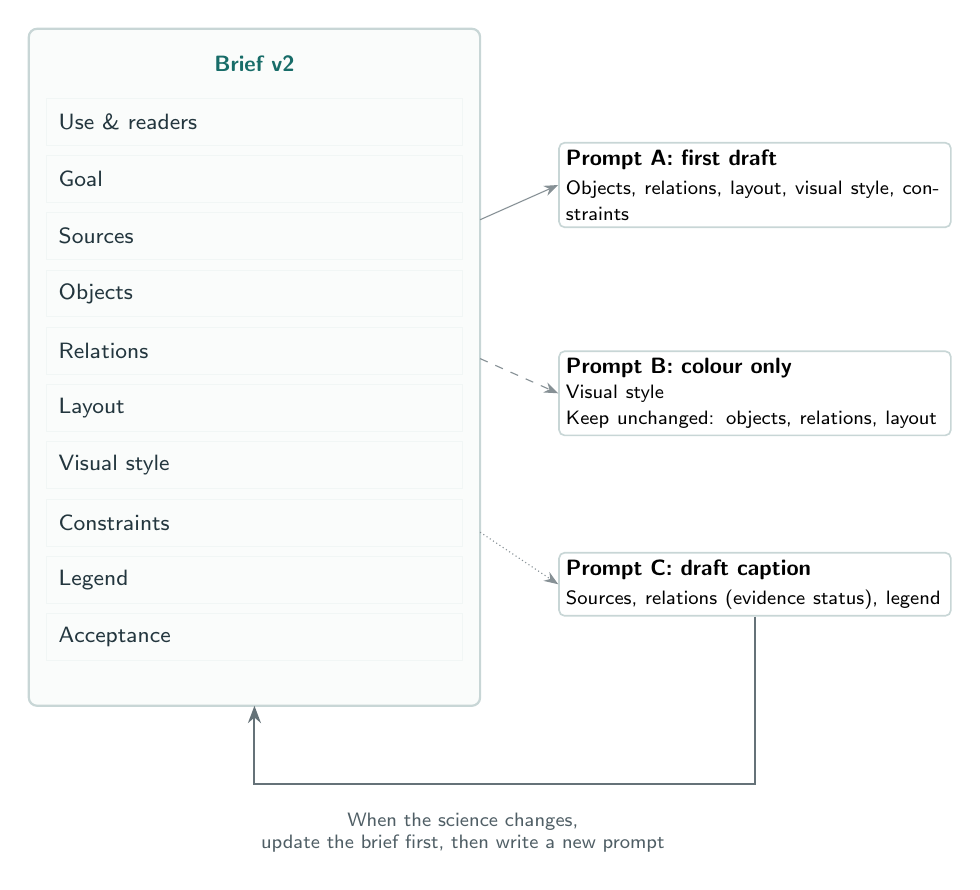
\begin{tikzpicture}[x=\linewidth/110,y=\linewidth/110]
\begin{scope}[
  font=\sffamily\footnotesize,
  field/.style={anchor=west, text=BookInk, inner sep=1.2pt},
  promptbox/.style={
    draw=BookRule, line width=0.6pt, rounded corners=2pt,
    fill=white, align=left, inner sep=2.5pt, text width=48mm,
  },
  conn/.style={draw=BookInk!55, thin},
]
  \def\briefW{52}
  \def\briefH{78}
  \coordinate (Bsw) at (0,0);
  \coordinate (Bne) at (\briefW,\briefH);
  \coordinate (aim) at (26,0);
  \draw[BookRule, line width=0.8pt, rounded corners=3pt, fill=BookPale!35]
    (Bsw) rectangle (Bne);
  \node[font=\sffamily\bfseries\footnotesize, text=BookTeal, anchor=north]
    at (0.5*\briefW,\briefH-2) {Brief v2};

  \foreach \j/\label in {
    1/Use \& readers,2/Goal,3/Sources,4/Objects,5/Relations,6/Layout,7/Visual style,8/Constraints,9/Legend,10/Acceptance} {
    \pgfmathsetmacro{\ytop}{\briefH - 8 - (\j-1)*6.6}
    \draw[BookPale, line width=0.4pt] (2,\ytop-5.4) rectangle (\briefW-2,\ytop);
    \node[field] at (3,\ytop-2.7) {\label};
  }

  \node[promptbox, anchor=west] (PA) at (61,60) {%
    \textbf{Prompt A: first draft}\\[1pt]
    \scriptsize Objects, relations, layout, visual style, constraints};
  \node[promptbox, anchor=west] (PB) at (61,36) {%
    \textbf{Prompt B: colour only}\\[1pt]
    \scriptsize Visual style\\
    \scriptsize Keep unchanged: objects, relations, layout};
  \node[promptbox, anchor=west] (PC) at (61,14) {%
    \textbf{Prompt C: draft caption}\\[1pt]
    \scriptsize Sources, relations (evidence status), legend};

  \draw[conn, -{Stealth[length=1.8mm]}] (\briefW,56) -- (PA.west);
  \draw[conn, dashed, -{Stealth[length=1.8mm]}] (\briefW,40) -- (PB.west);
  \draw[conn, densely dotted, -{Stealth[length=1.8mm]}] (\briefW,20) -- (PC.west);

  % Orthogonal return: down from Prompt C, left under the brief, up to its bottom edge.
  \coordinate (retLow) at (0,-9);
  \draw[BookInk!70, line width=0.7pt, -{Stealth[length=2.2mm]}]
    (PC.south) -- (PC.south |- retLow) -- (aim |- retLow) -- (aim);
  \node[font=\sffamily\scriptsize, text=BookInk!80, align=center, anchor=north, text width=58mm]
    at (50,-11.2) {When the science changes,\\update the brief first, then write a new prompt};
\end{scope}
\end{tikzpicture}

\newpage

\section*{ch02-03 paragraph-to-table (zh)}
\begin{table}[htbp]
\centering
% FIG ch02-03 paragraph to relation table (Chinese)
% Tabular only; input inside a table environment. No row colour:
% shared/preamble.tex loads xcolor without [table].
\begingroup
\setlength{\tabcolsep}{1.6pt}
\renewcommand{\arraystretch}{1}
\newcommand{\cellfont}{\fontsize{8}{9.3}\selectfont}
\newcommand{\gr}{\leavevmode\color{gray}}
\begin{tabularx}{\linewidth}{@{}
  >{\cellfont}l
  >{\cellfont}Y
  >{\cellfont\raggedright\arraybackslash}p{26mm}
  >{\cellfont\raggedright\arraybackslash}p{21mm}
  >{\cellfont\raggedright\arraybackslash}p{15.5mm}
@{}}
\toprule
\textbf{句} & \textbf{原句} & \textbf{图形表达} & \textbf{证据状态} & \textbf{是否画} \\
\midrule
S1 & 层状 NMC 正极（LiNi$_x$Mn$_y$Co$_z$O$_2$）的二次颗粒由大量初级晶粒团聚而成。
   & 颗粒剖面由多边形晶粒拼成
   & 确立（结构背景） & 画 \\
S2 & 在反复充放电中，初级晶粒随锂的脱出与嵌入发生各向异性的晶格膨胀与收缩，应力在晶界处积累，使二次颗粒内部沿晶界产生微裂纹（Ryu et al., 2018）。
   & 循环后颗粒内裂纹沿晶界分布
   & 确立（文献） & 画 \\
S3 & 裂纹让电解液渗入颗粒内部、暴露新的表面，并可能使部分碎块与导电网络失去接触，造成活性材料损失。
   & 裂纹内填浅蓝色电解液；颗粒边缘 1 块晶粒群轻微分离，叠加标签“活性材料损失”
   & 确立 & 画 \\
S4 & 在高荷电状态下，颗粒表面会由层状结构向类岩盐相重构并伴随晶格氧释放，形成的表面层使界面阻抗升高（Jung et al., 2017）。
   & 颗粒外表面一圈深色薄层；叠加标签“表面重构层 → 阻抗升高”
   & 确立（文献） & 画 \\
S5 & 与此同时，石墨负极表面的固体电解质界面膜（SEI）在循环中持续增厚，消耗可循环的锂，这通常是容量衰减的主要来源之一（Vetter et al., 2005; Birkl et al., 2017）。
   & 石墨颗粒外 SEI 由薄变厚；层间锂点变少，部分锂点嵌在 SEI 中
   & 确立（文献） & 画 \\
S6 & 我们推测，在本研究的电池中，裂纹新暴露表面上的电解液副反应也参与了阻抗的上升。
   & 叠加层中用虚线框和“推测”标签，从裂纹指向“阻抗升高”
   & 推测（虚线框） & 画，但区分 \\
\gr S7 & \gr 过渡金属溶出并在负极沉积，同样可能加速 SEI 生长，但不在本文讨论范围内。
   & \gr 图注写“未画：过渡金属溶出与沉积”
   & \gr 确立，但本文范围外 & \gr 不画 \\
\gr S8 & \gr 循环容量曲线见图 4。
   & \gr 示意图中不出现任何曲线、坐标轴、数值
   & \gr 数据，属于图 4 & \gr 不画 \\
\bottomrule
\end{tabularx}
\endgroup

\end{table}
\newpage

\section*{ch02-03 paragraph-to-table (en)}
\begin{table}[htbp]
\centering
% FIG ch02-03 paragraph to relation table (English)
% Tabular only; input inside a table environment. No row colour:
% shared/preamble.tex loads xcolor without [table].
\begingroup
\setlength{\tabcolsep}{1.6pt}
\renewcommand{\arraystretch}{1}
\newcommand{\cellfont}{\fontsize{8}{9.3}\selectfont}
\newcommand{\gr}{\leavevmode\color{gray}}
\begin{tabularx}{\linewidth}{@{}
  >{\cellfont}l
  >{\cellfont}Y
  >{\cellfont\raggedright\arraybackslash}p{26mm}
  >{\cellfont\raggedright\arraybackslash}p{21mm}
  >{\cellfont\raggedright\arraybackslash}p{15.5mm}
@{}}
\toprule
\textbf{Sent.} & \textbf{Sentence} & \textbf{Graphic expression} & \textbf{Evidence} & \textbf{Draw?} \\
\midrule
S1 & Secondary particles of a layered NMC cathode (LiNi$_x$Mn$_y$Co$_z$O$_2$) are agglomerates of many primary grains.
   & Polygonal grains in cross-section
   & Established (structural background) & Yes \\
S2 & During repeated cycling, the grains expand and contract anisotropically as lithium is extracted and reinserted; stress builds up at grain boundaries and opens intergranular microcracks inside the secondary particle (Ryu et al., 2018).
   & After cycling, cracks run along grain boundaries
   & Established (literature) & Yes \\
S3 & The cracks let electrolyte penetrate the particle and expose fresh surface, and some fragments may lose contact with the conductive network, causing loss of active material.
   & Pale-blue electrolyte in the cracks; one detached grain cluster; label ``loss of active material''
   & Established & Yes \\
S4 & At high states of charge, the particle surface reconstructs from the layered structure toward a rock-salt-like phase with release of lattice oxygen; the resulting surface layer raises interfacial impedance (Jung et al., 2017).
   & Thin dark outer rim; label ``reconstructed surface layer $\rightarrow$ higher impedance''
   & Established (literature) & Yes \\
S5 & Meanwhile, the solid electrolyte interphase (SEI) on the graphite anode keeps thickening during cycling and consumes cyclable lithium, which is commonly one of the main contributors to capacity fade (Vetter et al., 2005; Birkl et al., 2017).
   & SEI thickens; fewer lithium dots between layers, some embedded in the SEI
   & Established (literature) & Yes \\
S6 & We hypothesise that, in our cells, side reactions of the electrolyte on freshly exposed crack surfaces also contribute to the impedance rise.
   & Dashed box and ``hypothesis'' label, from the cracks to ``higher impedance''
   & Hypothesis (dashed box) & Yes, but distinct \\
\gr S7 & \gr Transition-metal dissolution and deposition on the anode may also accelerate SEI growth, but is outside the scope of this paper.
   & \gr Caption notes ``not shown: transition-metal dissolution and deposition''
   & \gr Established, out of scope & \gr No \\
\gr S8 & \gr The cycling capacity curves are shown in Figure 4.
   & \gr The schematic shows no curves, axes or values
   & \gr Data, Figure 4 & \gr No \\
\bottomrule
\end{tabularx}
\endgroup

\end{table}

\end{document}
